\chapter{Theoretical Aspects}

\noindent
The chapter serves as a comprehensive guide to the processes of conducting a study or development of new Generative Adversarial Networks. This is divided into two sections:

\begin{itemize}
    \item Research Methods and Data Collection, and
    \item Theoretical Explanation and Math behind GANs
\end{itemize}

% ----------------------------------------------------------

\section{Research Methods and Data Collection}

\noindent
Researchers employ a variety of methods in GAN-related studies, such as:
\begin{itemize}
    \item Collecting and Preprocessing Data
    \begin{itemize}
        \item Data Sources: Researchers start by collecting the data required for their specific GAN application. This data can be in various formats, including images, text, audio, or any other type of data relevant to the problem at hand.

        \item Data Preprocessing: Before feeding data into a GAN, it often requires preprocessing. This may involve tasks like data cleaning, normalization, resizing, and data augmentation to ensure that the data is suitable for training.
        
        \begin{itemize}
            \item Image Generation: In a study focused on generating realistic human faces, researchers collect a dataset of thousands of portrait images. These images are preprocessed to standardize the size, and crop faces, and adjust brightness and contrast to ensure uniform quality.
            \item Text Generation: For generating text using GANs, a text corpus of novels is collected. Preprocessing involves tokenization, removing punctuation, and lowercasing the text to create a clean and consistent dataset.
        \end{itemize}
    \end{itemize}
    
    \item Training GAN models using popular frameworks
    \begin{itemize}
        \item Researchers typically choose popular deep learning frameworks like TensorFlow, PyTorch, or Keras for developing and training GAN models. These frameworks offer a wide range of tools and resources for building and training neural networks, which are essential components of GANs.
        \item Architecture Selection: Depending on the specific GAN variant or the application, researchers choose the appropriate architecture for the generator and discriminator networks. For instance, they may opt for a Convolutional GAN for image generation tasks.
    \end{itemize}
    
    \item Fine-tuning models and optimizing hyperparameters.
    \begin{itemize}
        \item After initial training, researchers may perform fine-tuning, which is a crucial step to enhance the quality and diversity of generated data. This can involve adjusting parameters like learning rates, and batch sizes, adding regularization techniques and network architecture specifics to achieve the best performance. It is essential to ensure that the GAN meets the specific requirements of the task, whether it's generating high-resolution images, text, or any other content.
        \begin{itemize}
            \item Image Super-Resolution: After training a GAN to enhance image resolution, fine-tuning might involve adjusting the network architecture by adding skip connections or residual blocks to improve the visual quality of the generated high-resolution images.

            \item Conditional Text Generation: In text generation tasks, if researchers want to condition the GAN on specific attributes (e.g., genre for generating stories), they fine-tune the GAN by incorporating these conditions into the generator and discriminator networks.
        \end{itemize}

    \end{itemize}
\end{itemize}

% ----------------------------------------------------------

\section{Theoretical Explanation for GANs}

\noindent
This section embarks on a journey to delve deep into the core theoretical foundations and mathematical intricacies that underpin the remarkable success of Generative Adversarial Networks. Within this exploration, two main components of GANs, architecture, loss functions, training procedures, types of GANs, and practical applications are explained.

\begin{figure}[h!]
    \centering
    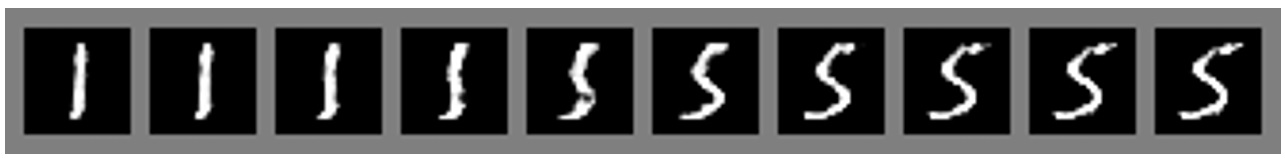
\includegraphics[width=0.8\textwidth]{Images/smooth_transition.jpg}
    \caption{Smooth transition of an image using GAN}
\end{figure}

\subsection{Components of GAN}

\noindent
At the core, GANs contain two main components:
\begin{itemize}
    \item The Generator, and
    \item The Discriminator
\end{itemize}

\noindent
The Generator: It is the creative element of the GAN. It takes random noise as input and transforms it into data samples. These samples can be anything from images to text. \textit{The primary objective of the generator is to produce data that is indistinguishable from real data}. In other words, the generator is responsible for creating new data(a.k.a fake data). It is implemented as a neural network, often a Deep Convolutional Neural Network(DCNN), which is well-suited for image generation tasks\cite{DCNN}.\\

\noindent
The Discriminator: The discriminator plays the role of a binary classifier. \textit{It evaluates whether a given data sample is real (from the training set) or fake (generated by the generator)}. In other words, the discriminator is responsible for distinguishing between real and fake data. Like the generator, the discriminator is also implemented as a neural network. Its goal is to become increasingly accurate at distinguishing real data from fake data over time.

\clearpage

\noindent
GANs were inspired by the game theory, more precisely, a zero-sum game, in which one's gain(+1) is the other's loss(-1), and the net outcome will be zero(+1-1 = 0). The generator and discriminator will compete with each other to achieve the Nash equilibrium(i.e. achieving the desired outcome not by deviating from the initial strategy) during its training process.\cite{GAN_Main}

\begin{figure}[h!]
    \centering
    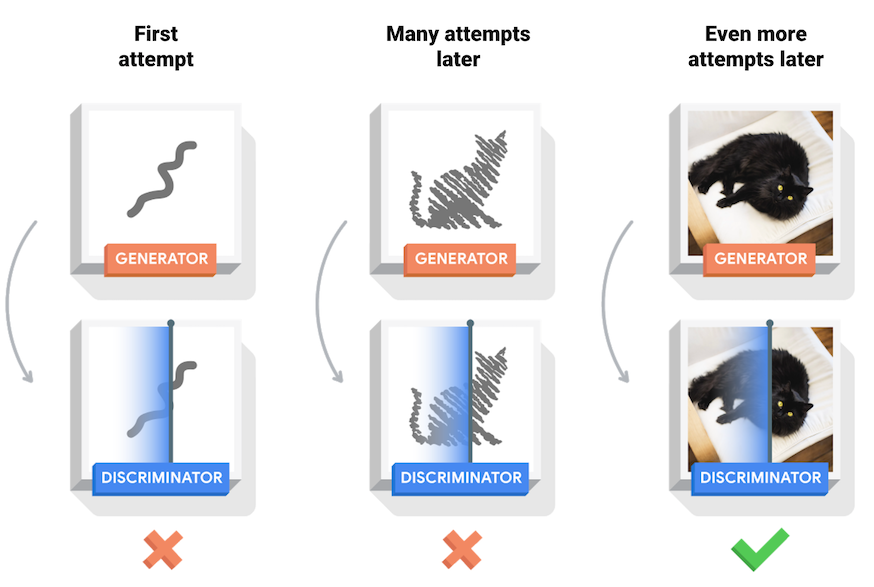
\includegraphics[width=\textwidth]{Images/gen_dis_working.png}
    \caption{Working of generator and discriminator}
\end{figure}

\noindent
Figure 3.2 depicts the working of the generator and discriminator in different attempts. At the beginning, the generator had no idea of what to create, so it made a doodle-like output. After many attempts, the generator has created a visually appealing and realistic image that is indistinguishable from the real image.

\clearpage

\subsection{Generator}

\begin{figure}[h!]
    \centering
    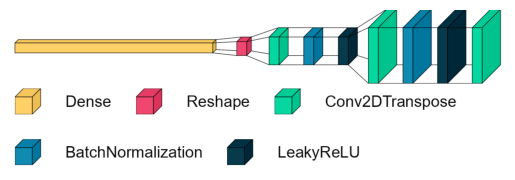
\includegraphics[width=0.9\textwidth]{Images/gen_arch.png}
    \caption{Generator Architecture}
\end{figure}

\noindent 
With the introduction of Deep Convolutional GAN by Radford, Chintala, et al. Convolutional Neural Networks have become the primary architecture for image generation tasks. Figure 3.3 shows a sample image of such image generation networks.

\begin{figure}[h!]
    \centering
    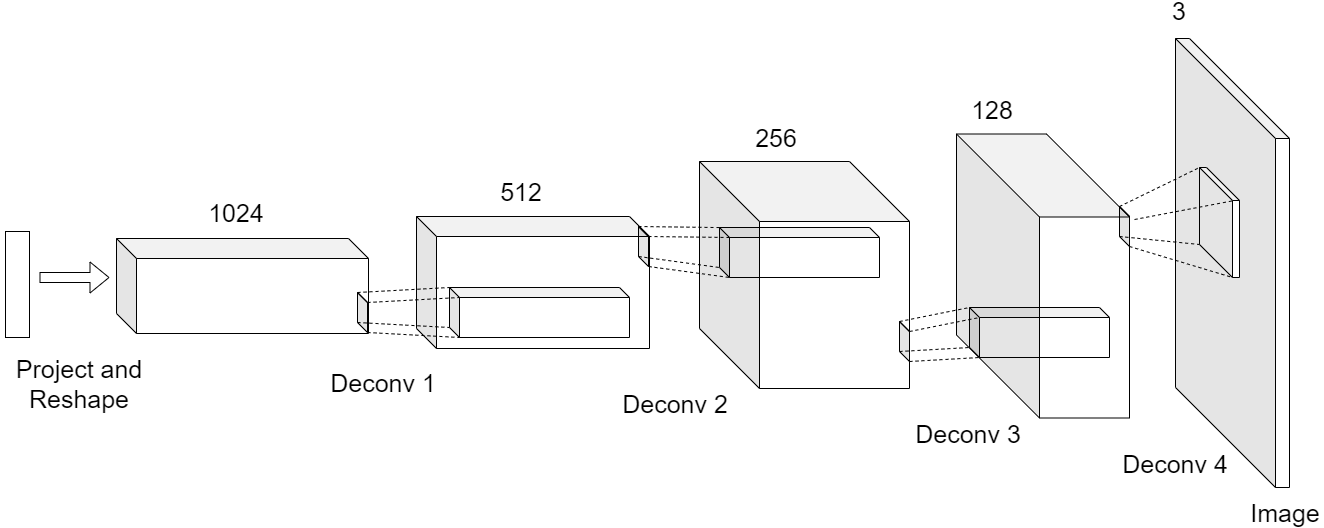
\includegraphics[width=\textwidth]{Images/deconvolution.png}
    \caption{Deconvolution Network used for upsampling in Generator}
\end{figure}

\noindent
Figure 3.4 depicts an Upsampling/Deconvolution Network, where it starts from a lower dimension, and becomes a clear and Full HD image at the end. 

\clearpage

\subsection{Discriminator}

\begin{figure}[h!]
    \centering
    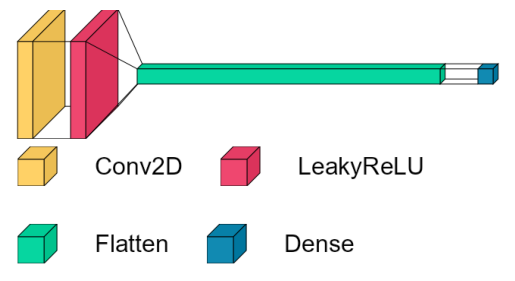
\includegraphics[width=0.9\textwidth]{Images/dis_arch.png}
    \caption{Discriminator Architecture}
\end{figure}

\noindent
The architecture of a discriminator is very similar to a normal binary classifier. It could use any network architecture appropriate to the type of data it's classifying. \\

\noindent
The discriminator will analyze the image using CNN layers and predict whether the image is real or fake (indicated by the integer value 1 or 0). The real example comes from the training dataset, and the generated examples are output by the generator model.\\

\noindent
In some advanced GAN variants, the discriminator may be designed to adapt to different levels of image quality, and it may provide more refined feedback to guide the generator's training.

\clearpage

% ---------------------------------------------------

\subsection{Architecture}

\noindent
The general architecture of GAN is a single diagram representing the training and testing process. Explanation for the architecture diagram (Figure 3.6):\\

\begin{figure}[h!]
    \centering
    \includegraphics[width=\textwidth]{Images/gan_arch.png}
    \caption{General Architecture of GAN}
\end{figure}

\noindent
First, the initialization is done with some random noise, it can be considered as a matrix of values that is taken from the training/testing data distribution. This random noise is given as the input of the generator, where the generator uses this random noise to create fake data.

\noindent
In the next step training sets and fake images are inputted to the discriminator during the training step. However, during the testing step, we only input the fake data created by the generator. During both phases, the discriminator has only one role, which is to identify whether the data given to it is real or fake. This output is given as an integer value of 1 or 0.

\noindent
The block diagram of the same architecture is given in Figure 3.7, it also depicts the same idea explained above. This diagram is the first point of reference for diagrams that will be shown in the GAN training section.

\clearpage

\begin{figure}[h!]
    \centering
    \includegraphics[width=\textwidth]{Images/gan_block_diag.png}
    \caption{Block Diagram of GAN}
\end{figure}

\noindent
The Generator will get its loss after the discriminator checks whether the created data is real or fake. The discriminator's loss depends on its output for the corresponding input of the generator. 

\subsection{Loss Function}

\noindent
The Standard GAN Loss Function is also known as the Min-Max Loss\cite{Nips_GAN}. This loss function is divided into Discriminator loss and Generator loss. The equation is given below, equation (1).
\[
\min_G \max_D V(D,G) = \mathbb{E}_{x \sim P_{\text{data}}(x)}[\log D(x)] + \mathbb{E}_{z \sim P_z(z)}[\log (1 - D(G(z)))]~-~(1)
\]

\noindent
Explanation for the terms in equation (1):
\begin{itemize}
    \item \textbf{E} represents the expected value or the average.
    \item \textbf{x} represents real data samples drawn from the real data distribution 
    \item \textbf{D(x)} is the output of Discriminator when it distinguishes real data from fake data.
    \item \textbf{z} represents random noise.
    \item \textbf{G(z)} is the output of the Generator when given random noise as input.
    \item \textbf{1-D(G(z))} represents the probability that the Discriminator assigns to the generated data being fake(1 minus the probability it assigns to it being real).
\end{itemize}

\clearpage

\noindent
The general GAN loss function is the sum of derived forms of discriminator and generator loss functions, which could be derived using the general equation of Binary Cross-Entropy, which is given by
\[
L(y,\hat{y}) = -\left(y\cdot \log_{}\hat{y} + (1-y)\cdot \log_{}(1-\hat{y})\right)~-~(2)
\]

\noindent
Where \textbf{L(y, $\mathbf{\hat{y}}$)} is the loss.

\noindent
We substitute y = 1 for real images and y = 0 for fake images in the Binary Cross-Entropy equation, to get:
\[
L(\text{Discriminator}) = \min\left[-\left(\log_{}(D(x)) + \log_{}(1-D(G(z)))\right)\right]~-~(3)
\]

\noindent
Removing the negative sign will change min to max:
\[
L(\text{Discriminator}) = \max\left[\log_{}(D(x)) + \log_{}(1-D(G(z)))\right]~-~(4)
\]

\noindent
Maximizing the loss function means to put D(x) = 1, and D(G(z)) = 0. So, the loss function will result in 0 (Fake image).

\noindent
Note: \textbf{log(1) = 0}

\noindent
Generator loss is calculated from the discriminator loss. The generator will try to fool the discriminator into classifying the fake data as real data. This implies that the generator tries to minimize the second term in the discriminator loss equation.
\[
L(\text{Generator}) = \min\left[\log_{}(1-D(G(z)))\right]~-~(5)
\]

\noindent
Minimizing the loss function means to put D(G(z)) = close to 1. So, the loss function will result in 1 (Real image).\\

\noindent
By taking the sum of both the equations (4) \& (5), we get the general equation for the GAN loss function back, equation (6):
\[
\min_G \max_D V(D,G) = \mathbb{E}_{x\sim P_{\text{data}}(x)}\left[\log_{}D(x)\right] + \mathbb{E}_{z\sim P_z(z)}\left[\log_{}(1-D(G(z)))\right]~-~(1)
\]

\clearpage

\subsection{Training}

\noindent
The training of GANs has three main phases:
\begin{itemize}
    \item The starting of training
    \item The Optimal training time, and
    \item The stopping of training
\end{itemize}

\noindent
The GAN starts training in alternating periods. The discriminator trains for one or more epochs then the generator’s turn and this step repeats. Careful training is required, as most challenges of GANs are in the training phase.\\

\noindent
The optimal training duration will depend on: 
\begin{itemize}
    \item Complexity of the data being generated
    \item Size of the training dataset, and
    \item The desired quality of the generated data.
\end{itemize}

\noindent
The training can be stopped when:
\begin{itemize}
    \item The generator is able to produce high-quality samples that are identical to real data.
    \item The discriminator is no longer able to classify real and fake data with high accuracy.
\end{itemize}

\subsection{Generator Training}

\noindent
In a typical Generative Adversarial Network training process, random noise is first fed into the generator, which produces a synthetic data sample. This generated sample is then passed to the discriminator, whose role is to classify whether the sample is real or fake. The discriminator is kept constant during the generator training phase. Otherwise, the generator would try to hit a target (output of discriminator) and never converge. The discriminator's classification forms the basis for calculating the loss, quantifying the difference between the discriminator's predictions and the actual labels (real or fake). 

\clearpage

\noindent
This loss is backpropagated through both the discriminator and the generator to obtain gradients, which describe the direction and magnitude of the necessary weight adjustments. However, it's crucial to note that during this training phase, these gradients are used exclusively to modify the generator's weights. This adversarial interplay between the generator and the discriminator continues iteratively, with the generator aiming to produce increasingly realistic data while the discriminator seeks to become more selective, ultimately leading to improved GAN performance.

\begin{figure}[h!]
    \centering
    \includegraphics[width=\textwidth]{Images/gen_training.png}
    \caption{Generator Training}
\end{figure}

\subsection{Discriminator Training}

\noindent
In the discriminator training process, a fake image generated by the generator is passed to the discriminator. The discriminator's role is to classify whether the image is real (from the true data distribution) or fake (generated by the generator). During discriminator training, the generator is paused. Its weights remain constant while it produces examples for the discriminator to train on. Based on this classification, a loss is calculated, quantifying how well the discriminator is distinguishing between real and fake images. The gradients of this loss are then obtained through backpropagation and used to adjust the discriminator's weights. This iterative process helps the discriminator become better at distinguishing real from fake images.

\clearpage

\begin{figure}[h!]
    \centering
    \includegraphics[width=\textwidth]{Images/dis_training.png}
    \caption{Discriminator Training}
\end{figure}

\subsection{Types of GANs}

\begin{table}[h!]
    \centering
    \caption{Types of GANs with Specializations}
    \begin{tabular}{|c|c|}
    \hline
    \textbf{GAN Type} & \textbf{Specialization} \\ 
    \hline
    Normal GAN & Basic GAN architecture for image generation \\
    \hline
    CGAN & Controlled image generation(conditional inputs) \\
    \hline
    DCGAN & Deep Convolutional GAN for image generation \\
    \hline
    StyleGAN & High-quality image synthesis with style control \\
    \hline
    BigGAN\cite{BigGAN} & High-quality images at high resolutions\\
    \hline
    MuseGAN\cite{MuseGAN} & Music Generation using GAN \\
    \hline
    DiscoGAN\cite{DiscoGAN} & Learn cross-domain relations in unsupervised data.\\
    \hline
    CycleGAN\cite{CycleGAN} & Unpaired image-to-image translation \\
    \hline
    SocialGAN\cite{SocialGAN} & Socially Acceptable Trajectories with GAN \\
    \hline
    ProgressiveGAN(PGAN)\cite{PGAN} & Training GANs for high-resolution images \\
    \hline
    Self-AttentionGAN(SAGAN) & Self-attention mechanism for image generation \\
    \hline
    WassersteinGAN(WGAN)\cite{WGAN} & Enhanced stability and training by Wasserstein loss \\
    \hline
    \end{tabular}
\end{table}

\clearpage

\noindent
Even though there are different types of GANs, the focus is only on the Conditional Generative Adversarial Networks because it is used in the research work, which is going to be explored in the next chapter.\\

\noindent
The CGAN is used because, in traditional GAN, the user has no control over the modes of the data to be generated. But conditional GAN changes that by adding the label 'y' as an additional parameter to the generator to generate specified images. Also, the label is added to the discriminator to distinguish real images better. See the mathematical equation differences:

\noindent
The general loss function equation, same equation as given above (equation(1)) for GAN is given by,
\[
\min_G \max_D V(D,G) = \mathbb{E}_{x\sim P_{\text{data}}(x)}\left[\log_{}D(x)\right] + \mathbb{E}_{z\sim P_z(z)}\left[\log_{}(1-D(G(z)))\right]~-~(1)
\]

\noindent
The equation for CGAN is given by,
\[
\min_G \max_D V(D,G) = \mathbb{E}_{x\sim P_{\text{data}}(x)}\left[\log_{}D(x|y)\right] + \mathbb{E}_{z\sim P_z(z)}\left[\log_{}(1-D(G(z|y)))\right]~-~(6)
\]

\noindent
In equation (6) \textbf{y} term is a new addition, which is used to control the output of CGAN.

\begin{figure}[h!]
    \centering
    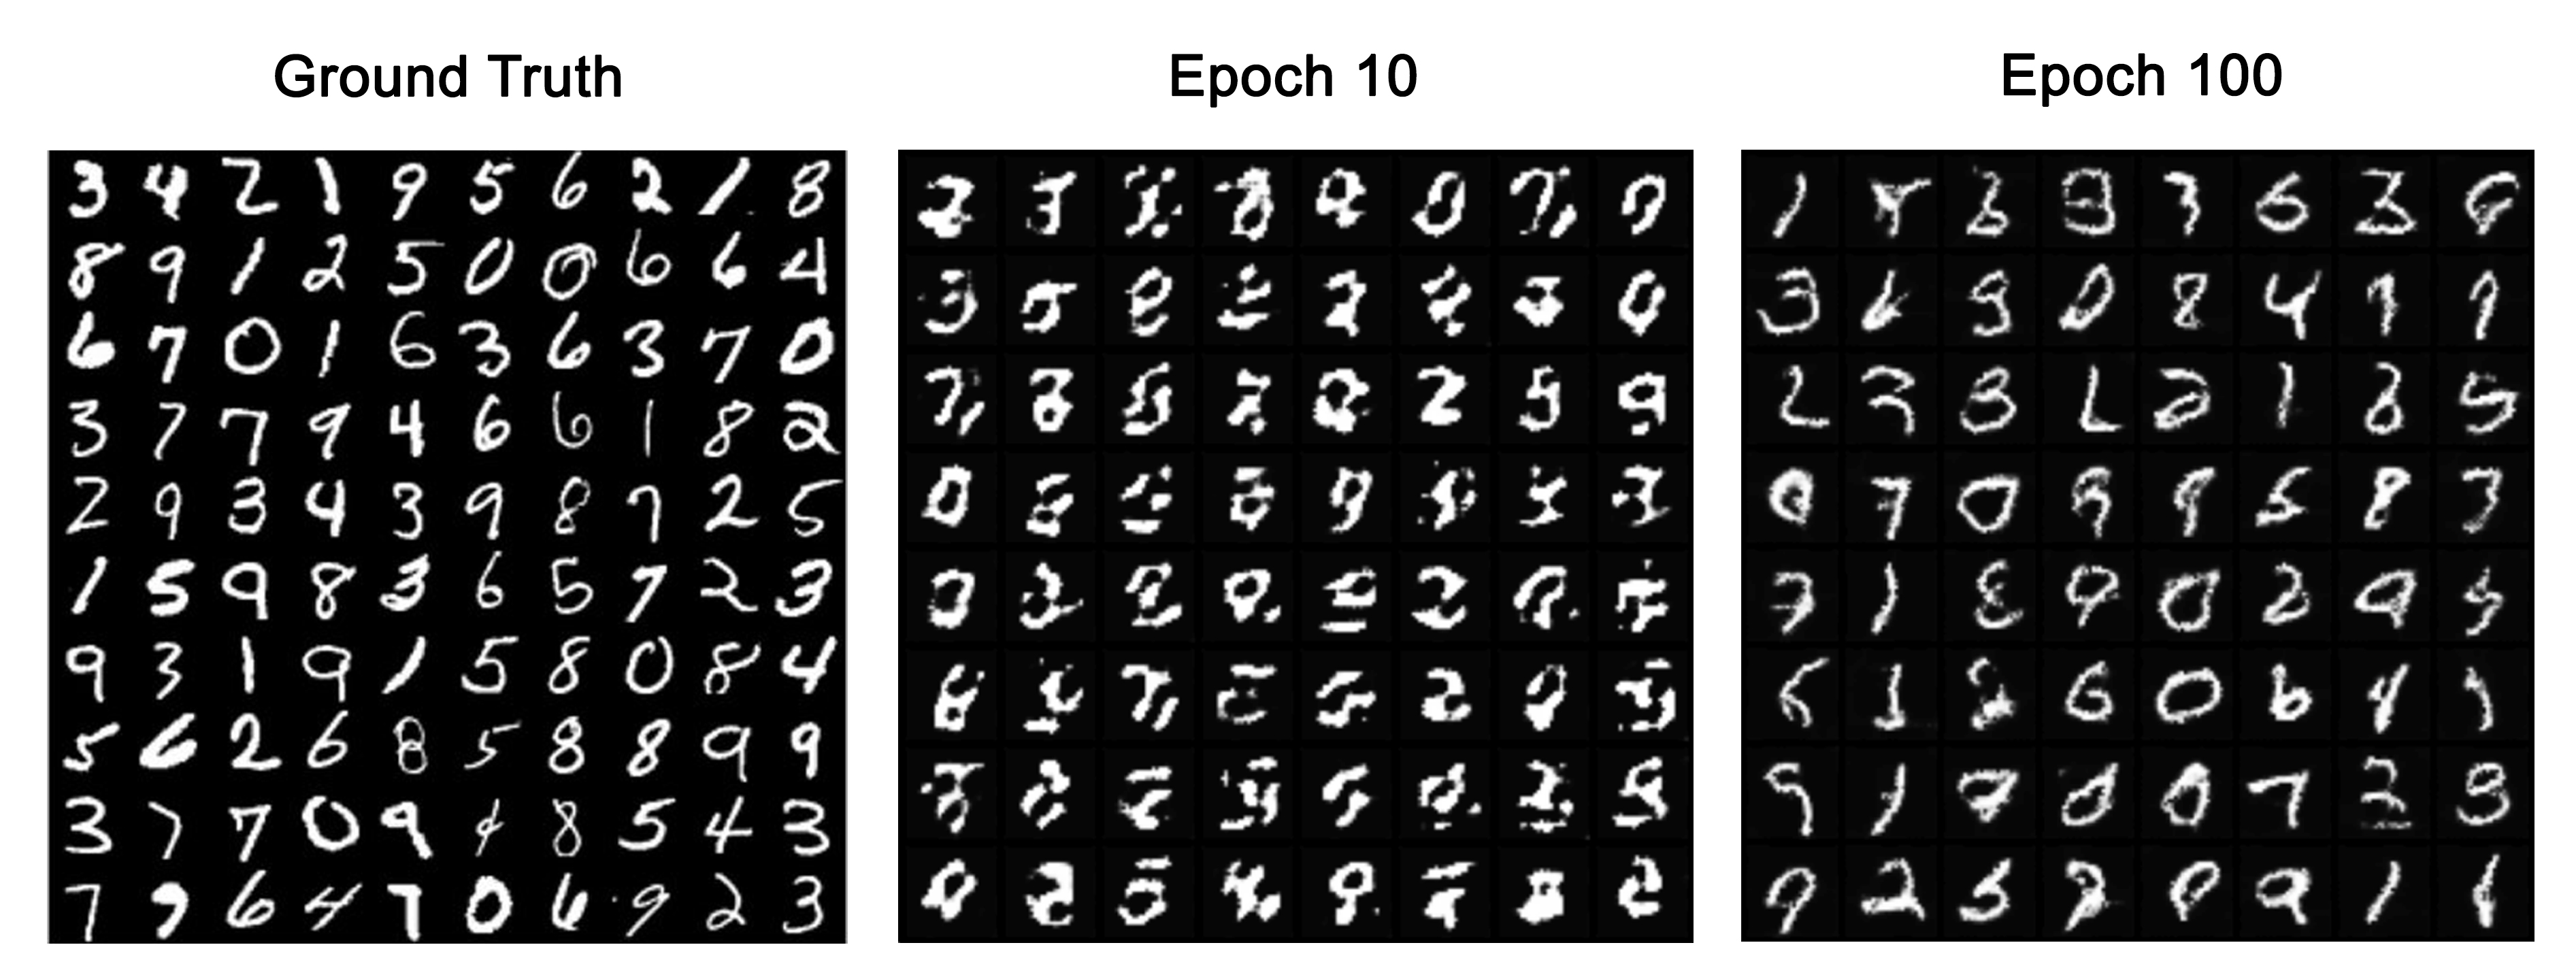
\includegraphics[width=\textwidth]{Images/gan_mnist.jpg}
    \caption[GAN working on MNIST Data]{GAN working on MNIST Data\cite{GAN_Main}}
\end{figure}

\clearpage

\subsection{Uses of GANs}

\begin{table}[h!]
\centering
\caption{Uses of GANs}
\begin{tabular}{|c|c|c|}
\hline
\textbf{Application} & \textbf{GAN Type} & \textbf{Description} \\
\hline
Image Generation & Vanilla GAN & Realistic images from noise \\
\hline
Style Transfer & CycleGAN & Apply artistic styles to photos \\
\hline
Face Aging & Face Aging GAN\cite{Face_Aging_GAN} & Simulate the aging process of faces \\
\hline
Data Augmentation & DCGAN & Training data for ML models \\
\hline
Video Generation & VideoGAN\cite{VideoGAN} & Synthetic video sequences \\
\hline
Drug Discovery & ChemGAN\cite{ChemGAN} & Molecular structures for drug design \\
\hline
\end{tabular}
\end{table}

\noindent
In addition to Table 3.2, Figure 3.11 will give a pie-chart representation of the use of GAN in the industry.\\

\begin{figure}[h!]
    \centering
    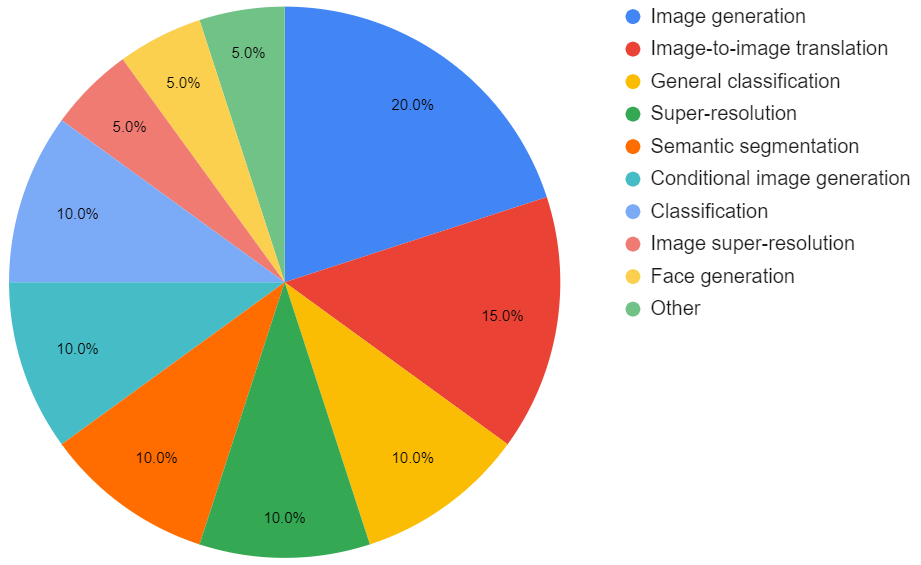
\includegraphics[width=\textwidth]{Images/gan_use.png}
    \caption{Uses of GAN as Pie-Chart}
\end{figure}

\clearpage

\noindent
In a nutshell, Generative Adversarial Networks are a powerful type of deep learning model that can be used to generate new data, such as images, text, and music\cite{DCGAN}\cite{CORRGAN}\cite{MuseGAN}. The GAN is trained using two neural networks: a generator and a discriminator. The generator creates new data, and the discriminator tries to distinguish between real and generated data.\cite{Nips_GAN} The generator and discriminator are trained in a competitive manner, where the generator tries to fool the discriminator, and the discriminator tries to become better at distinguishing between real and generated data.\cite{GAN_Main}

\noindent
Figure 3.11 illustrates a classical example usage of GANs to regenerate Modified National Institute of Standards and Technology(MNIST) Data. MNIST is a dataset of handwritten digits, commonly known as \textit{Hello World to Deep Learning}. The figure shows the GAN at two different epochs: 10 and 100. At epoch 10, the generator is still learning how to generate realistic MNIST digits. The generated digits are often blurry and deformed. However, by epoch 100, the generator has learned to generate much more realistic MNIST digits. The generated digits are now sharp and well-defined.\\

\noindent
There are many specialized GANs that have been developed for specific tasks, such as DCGAN(Image Generation) designed for generating high-quality synthetic images, StyleGAN(Human Face Generation) generating high-resolution human faces with a high degree of variability and realism, StarGAN(Style Transfer)\cite{StarGAN}, which is capable of performing style transfer across multiple domains. For instance, it can convert the style of an image from one domain (e.g., one type of facial expression) to another (e.g., a different facial expression)., and SemanticGAN (Semantic Segmentation)\cite{SemanticGAN}, it is oriented toward semantic segmentation, a task in computer vision that involves classifying each pixel in an image into a specific category, such as object detection or image segmentation. These models are also used to develop new types of applications like Artbreeder, DeepFace, Prisma, FacePlay, MidJourney, and DALL·E.